%%%%%%%%%%%%%%%%%%%%%%%%%%%%%%%%%%%%%%%%%
% Thin Sectioned Essay
% LaTeX Template
% Version 1.0 (3/8/13)
%
% This template has been downloaded from:
% http://www.LaTeXTemplates.com
%
% Original Author:
% Nicolas Diaz (nsdiaz@uc.cl) with extensive modifications by:
% Vel (vel@latextemplates.com)
%
% License:
% CC BY-NC-SA 3.0 (http://creativecommons.org/licenses/by-nc-sa/3.0/)
%
%%%%%%%%%%%%%%%%%%%%%%%%%%%%%%%%%%%%%%%%%

%----------------------------------------------------------------------------------------
%	PACKAGES AND OTHER DOCUMENT CONFIGURATIONS
%----------------------------------------------------------------------------------------

\documentclass[a4paper, 12pt]{article} % Font size (can be 10pt, 11pt or 12pt) and paper size (remove a4paper for US letter paper)

\usepackage[protrusion=true,expansion=true]{microtype} % Better typography
\usepackage{graphicx} % Required for including pictures
\usepackage[utf8]{inputenc}
\usepackage[margin=1.0in]{geometry}
\usepackage{url}
\usepackage{fancyhdr}
\usepackage{amsmath}
\usepackage{setspace}
\usepackage{enumitem}
\usepackage{float}
\setlength\parindent{0pt} % Removes all indentation from paragraphs

\usepackage[T1]{fontenc} % Required for accented characters
\usepackage{times} % Use the Palatino font

\usepackage{listings}
\usepackage{color}
\lstset{mathescape}

\definecolor{dkgreen}{rgb}{0,0.6,0}
\definecolor{gray}{rgb}{0.5,0.5,0.5}
\definecolor{mauve}{rgb}{0.58,0,0.82}

\lstset{frame=tb,
   language=c++,
   aboveskip=3mm,
   belowskip=3mm,
   showstringspaces=false,
   columns=flexible,
   basicstyle={\small\ttfamily},
   numbers=none,
   numberstyle=\tiny\color{gray},
   keywordstyle=\color{blue},
   commentstyle=\color{dkgreen},
   stringstyle=\color{mauve},
   breaklines=true,
   breakatwhitespace=true
   tabsize=3
}
\linespread{1.00} % Change line spacing here, Palatino benefits from a slight increase by default

\makeatletter
\renewcommand{\@listI}{\itemsep=0pt} % Reduce the space between items in the itemize and enumerate environments and the bibliography

\renewcommand\abstractname{Résumé}
\renewcommand\refname{Références}
\renewcommand\contentsname{Table des matières}
\renewcommand{\maketitle}{ % Customize the title - do not edit title and author name here, see the TITLE block below
\begin{center} % Right align

\vspace*{25pt} % Some vertical space between the title and author name
{\LARGE\@title} % Increase the font size of the title

\vspace{125pt} % Some vertical space between the title and author name

{\large\@author} % Author name

\vspace{125pt} % Some vertical space between the author block and abstract
Dans le cadre du cours
\\INF8225 - Techniques probabilistes et d'apprentissage
\vspace{125pt} % Some vertical space between the author block and abstract
\\\@date % Date
\vspace{125pt} % Some vertical space between the author block and abstract

\end{center}
}

%----------------------------------------------------------------------------------------
%	TITLE
%----------------------------------------------------------------------------------------

\title{TP2: } 

\author{\textsc{Guillaume Arruda 1635805} % Author
\vspace{10pt}
\\{\textit{École polytechnique de Montréal}}} % Institution

\date{19 Février 2016} % Date

%----------------------------------------------------------------------------------------

\begin{document}

\thispagestyle{empty}
\clearpage\maketitle % Print the title section
\pagebreak[4]
%----------------------------------------------------------------------------------------
%	En tête et pieds de page 
%----------------------------------------------------------------------------------------

\setlength{\headheight}{15.0pt}
\pagestyle{fancy}
\fancyhead[L]{INF8225}
\fancyhead[C]{}
\fancyhead[R]{TP2}
\fancyfoot[C]{\textbf{page \thepage}}

%----------------------------------------------------------------------------------------
%	ESSAY BODY
%----------------------------------------------------------------------------------------
\section*{Partie 1}
La première partie de ce laboratoire consistait à implémenter deux techniques matriciels de régression logistique et les comparer. La première technique est l'approche par "Batch" où toutes les
données d'apprentissage sont utilisé pour calculer le gradient et mettre à jour les poids. Le seconde technique est l'approche par "Mini-Batch" où les données d'apprentissages sont séparées en
plusieurs groupes et le calcul du gradient est effectué au traitement de chaqu'un des groupes.
\begin{figure}[H]
\label{learningCurves}
\caption{Courbes d'apprentissages des techniques Batch et miniBatches}
\includegraphics[width=\textwidth,height=\textheight,keepaspectratio]{graphics/learningCurves.eps}
\end{figure}

La figure~\ref{learningCurves} montre la précision des deux techniques en fonctions du nombre d'itération et de l'échantillon mesuré. Il est possible de voir que, pour les deux techniques, la 
précision sur l'ensemble de test est toujours meilleurs que la précision sur l'ensemble de validation. Ceci est un résultat attendu, car les algorithmes ont appris sur l'ensemble de test et sont 
donc plus performant sur celui. L'apprentissage par "Mini-Batch" est beaucoup plus rapide à converger que l'algorithme par "Batch", mais ne réussi pas à être aussi précis que celui-ci.
\begin{figure}[H]
\label{logVraisemblance}
\caption{LogVraisemblance des techniques Batch et miniBatches}
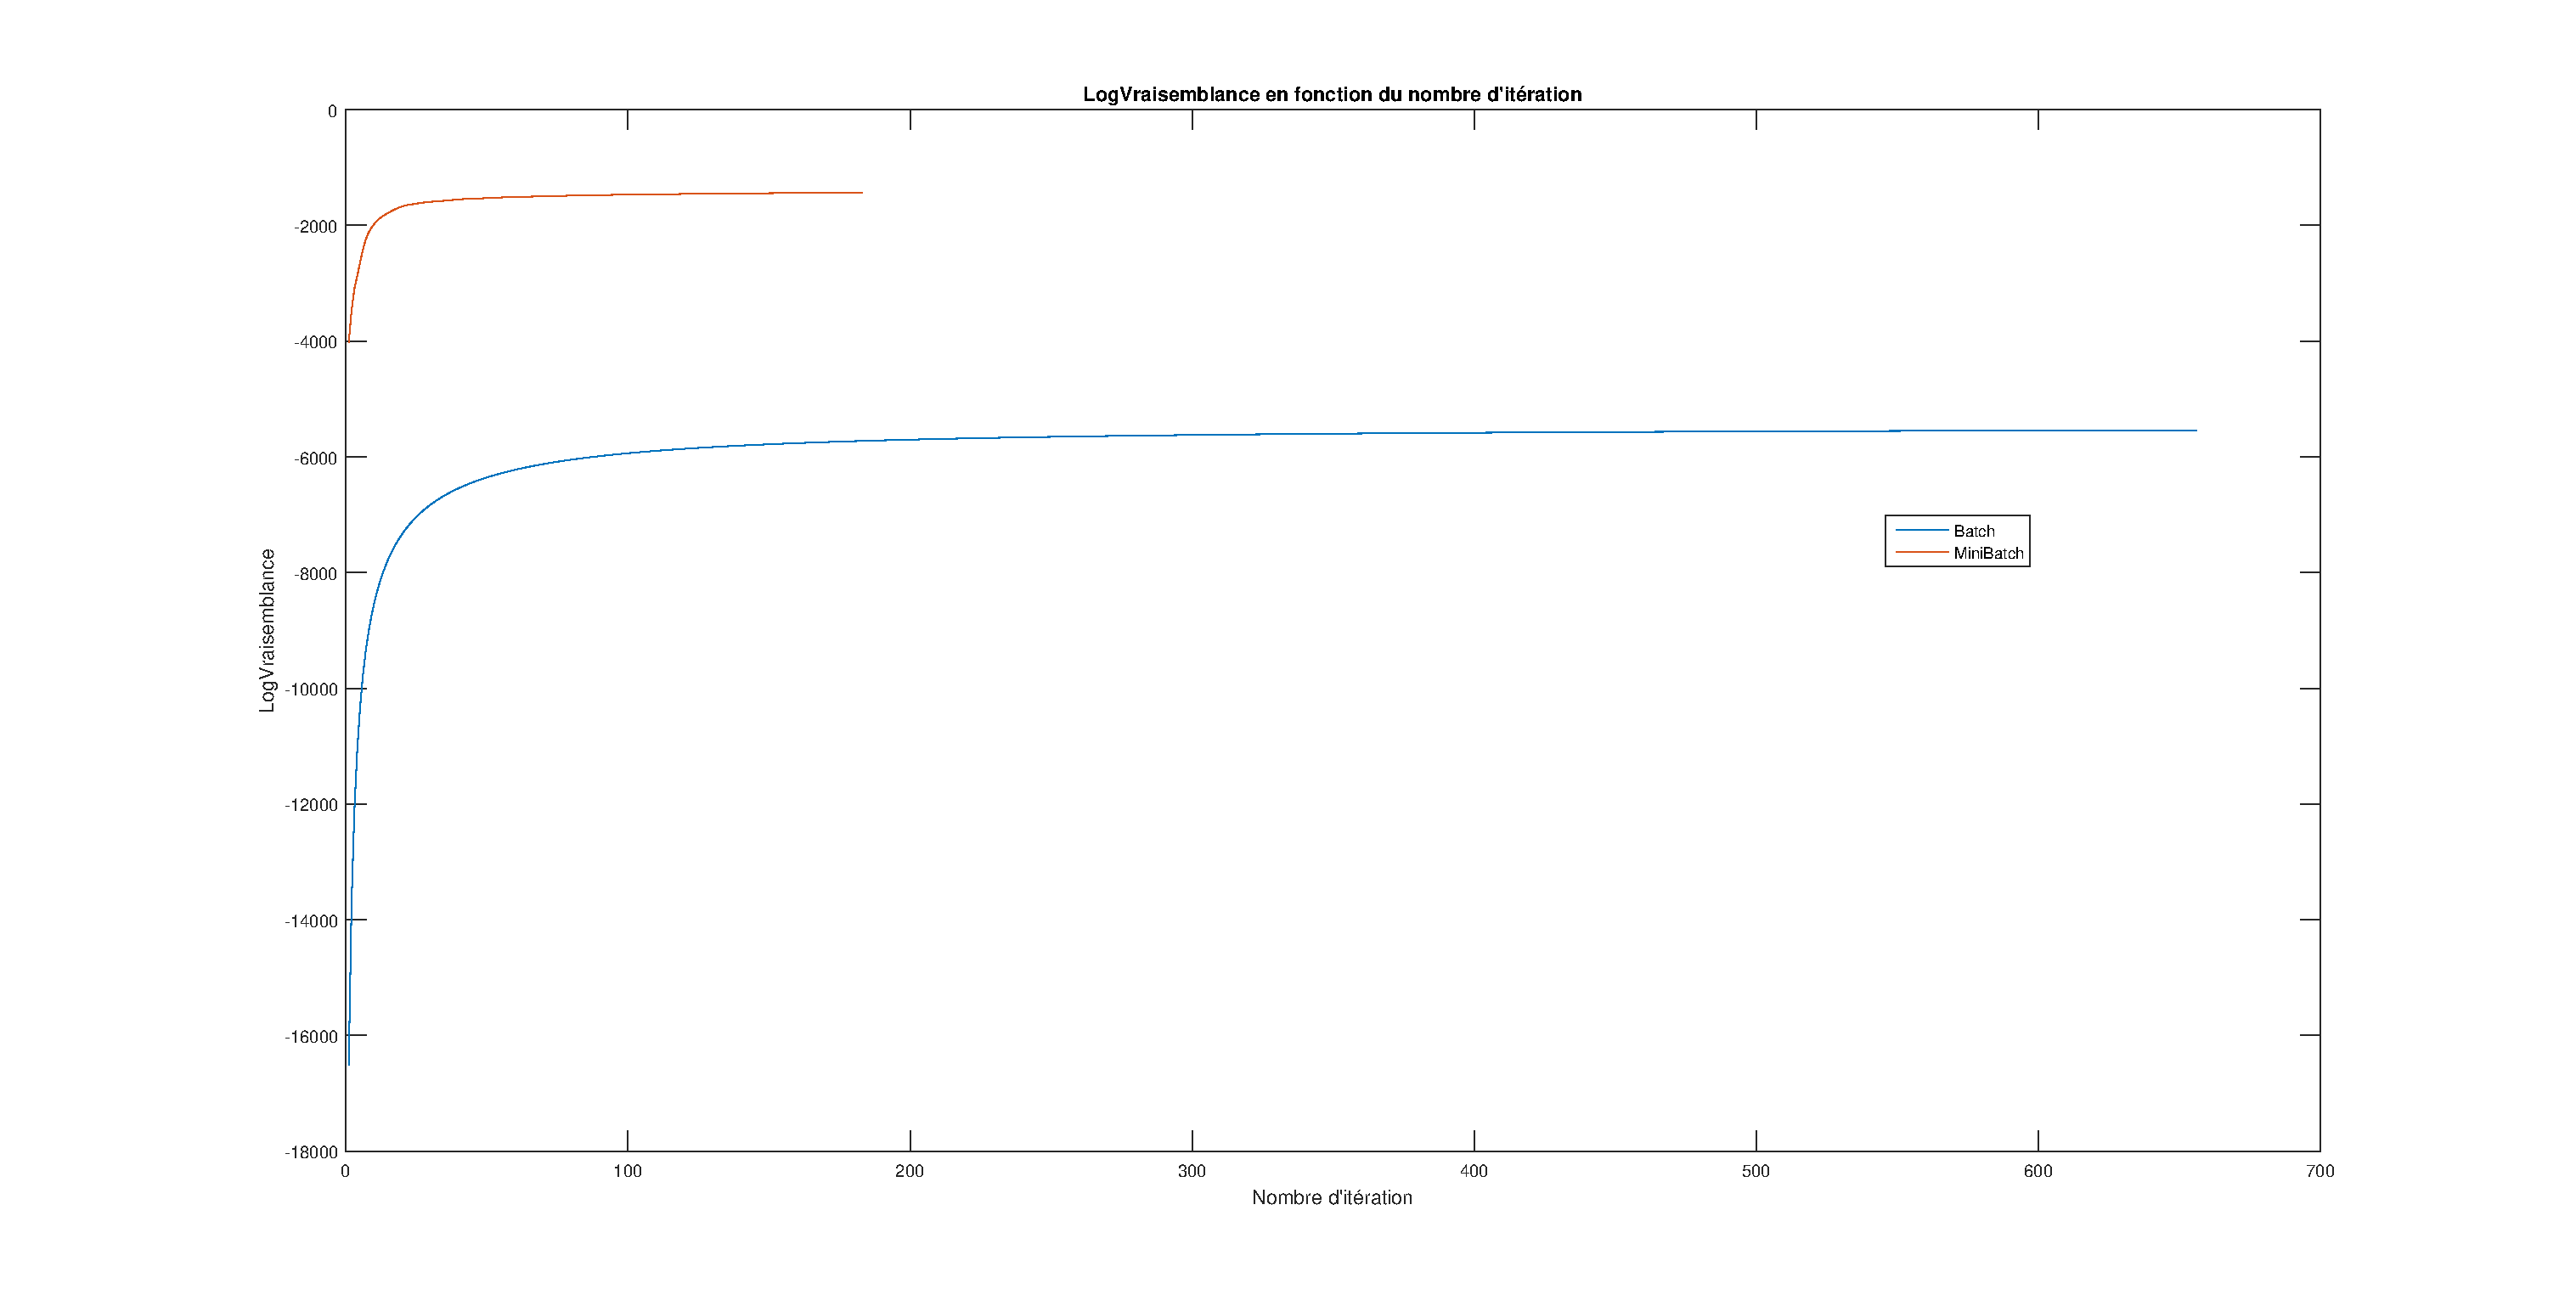
\includegraphics[width=\textwidth,height=\textheight,keepaspectratio]{graphics/logValidityCurves.eps}
\end{figure}

\section*{Partie 2}
La deuxième partie de ce laboratoire consistait à ajouter un terme de régularisation de type "Élastic Net" à l'apprentissage par "Mini-Batch". Pour tester l'éfficacité de se terme, 100 variables aléatoires
ont été rajouté aux données.
\begin{figure}[H]
\label{weightNoRegulation}
\caption{Valeur absolue du poids des paramètres valides sans régulation}
\includegraphics[width=\textwidth,height=\textheight,keepaspectratio]{graphics/histoValidParameterNoRegulation.eps}
\end{figure}

\begin{figure}[H]
\label{weightRegulation}
\caption{Valeur absolue du poids des paramètres valides avec régulation}
\includegraphics[width=\textwidth,height=\textheight,keepaspectratio]{graphics/histoValidParameterRegulation.eps}
\end{figure}

Aux niveau des paramètres valides des données, le terme de régulation a fait tendre les valeurs des poids vers 0. Plusieurs paramètre qui avait autrefois des valeurs entre 0 et 1, ont vu leur poids diminuer
à 0. Le terme de régulation à donc permis de voir plus clairement quelle variable avait un effet sur quel sortie et pourrait même permettre d'éliminer complétement une entrée si celle-ci n'a aucun effet sur 
la sortie. Le terme de régulation, même s'il a descendu la précision d'environ 4\% permet de trouver les entrées inutiles et donc de les retirer des calculs. Cela permet donc d'accélerer les calculs et de 
réduire le coût de la collecte de données.

\begin{figure}[H]
\label{randomWeightNoRegulation}
\caption{Valeur absolue du poids des paramètres aléatoires sans régulation}
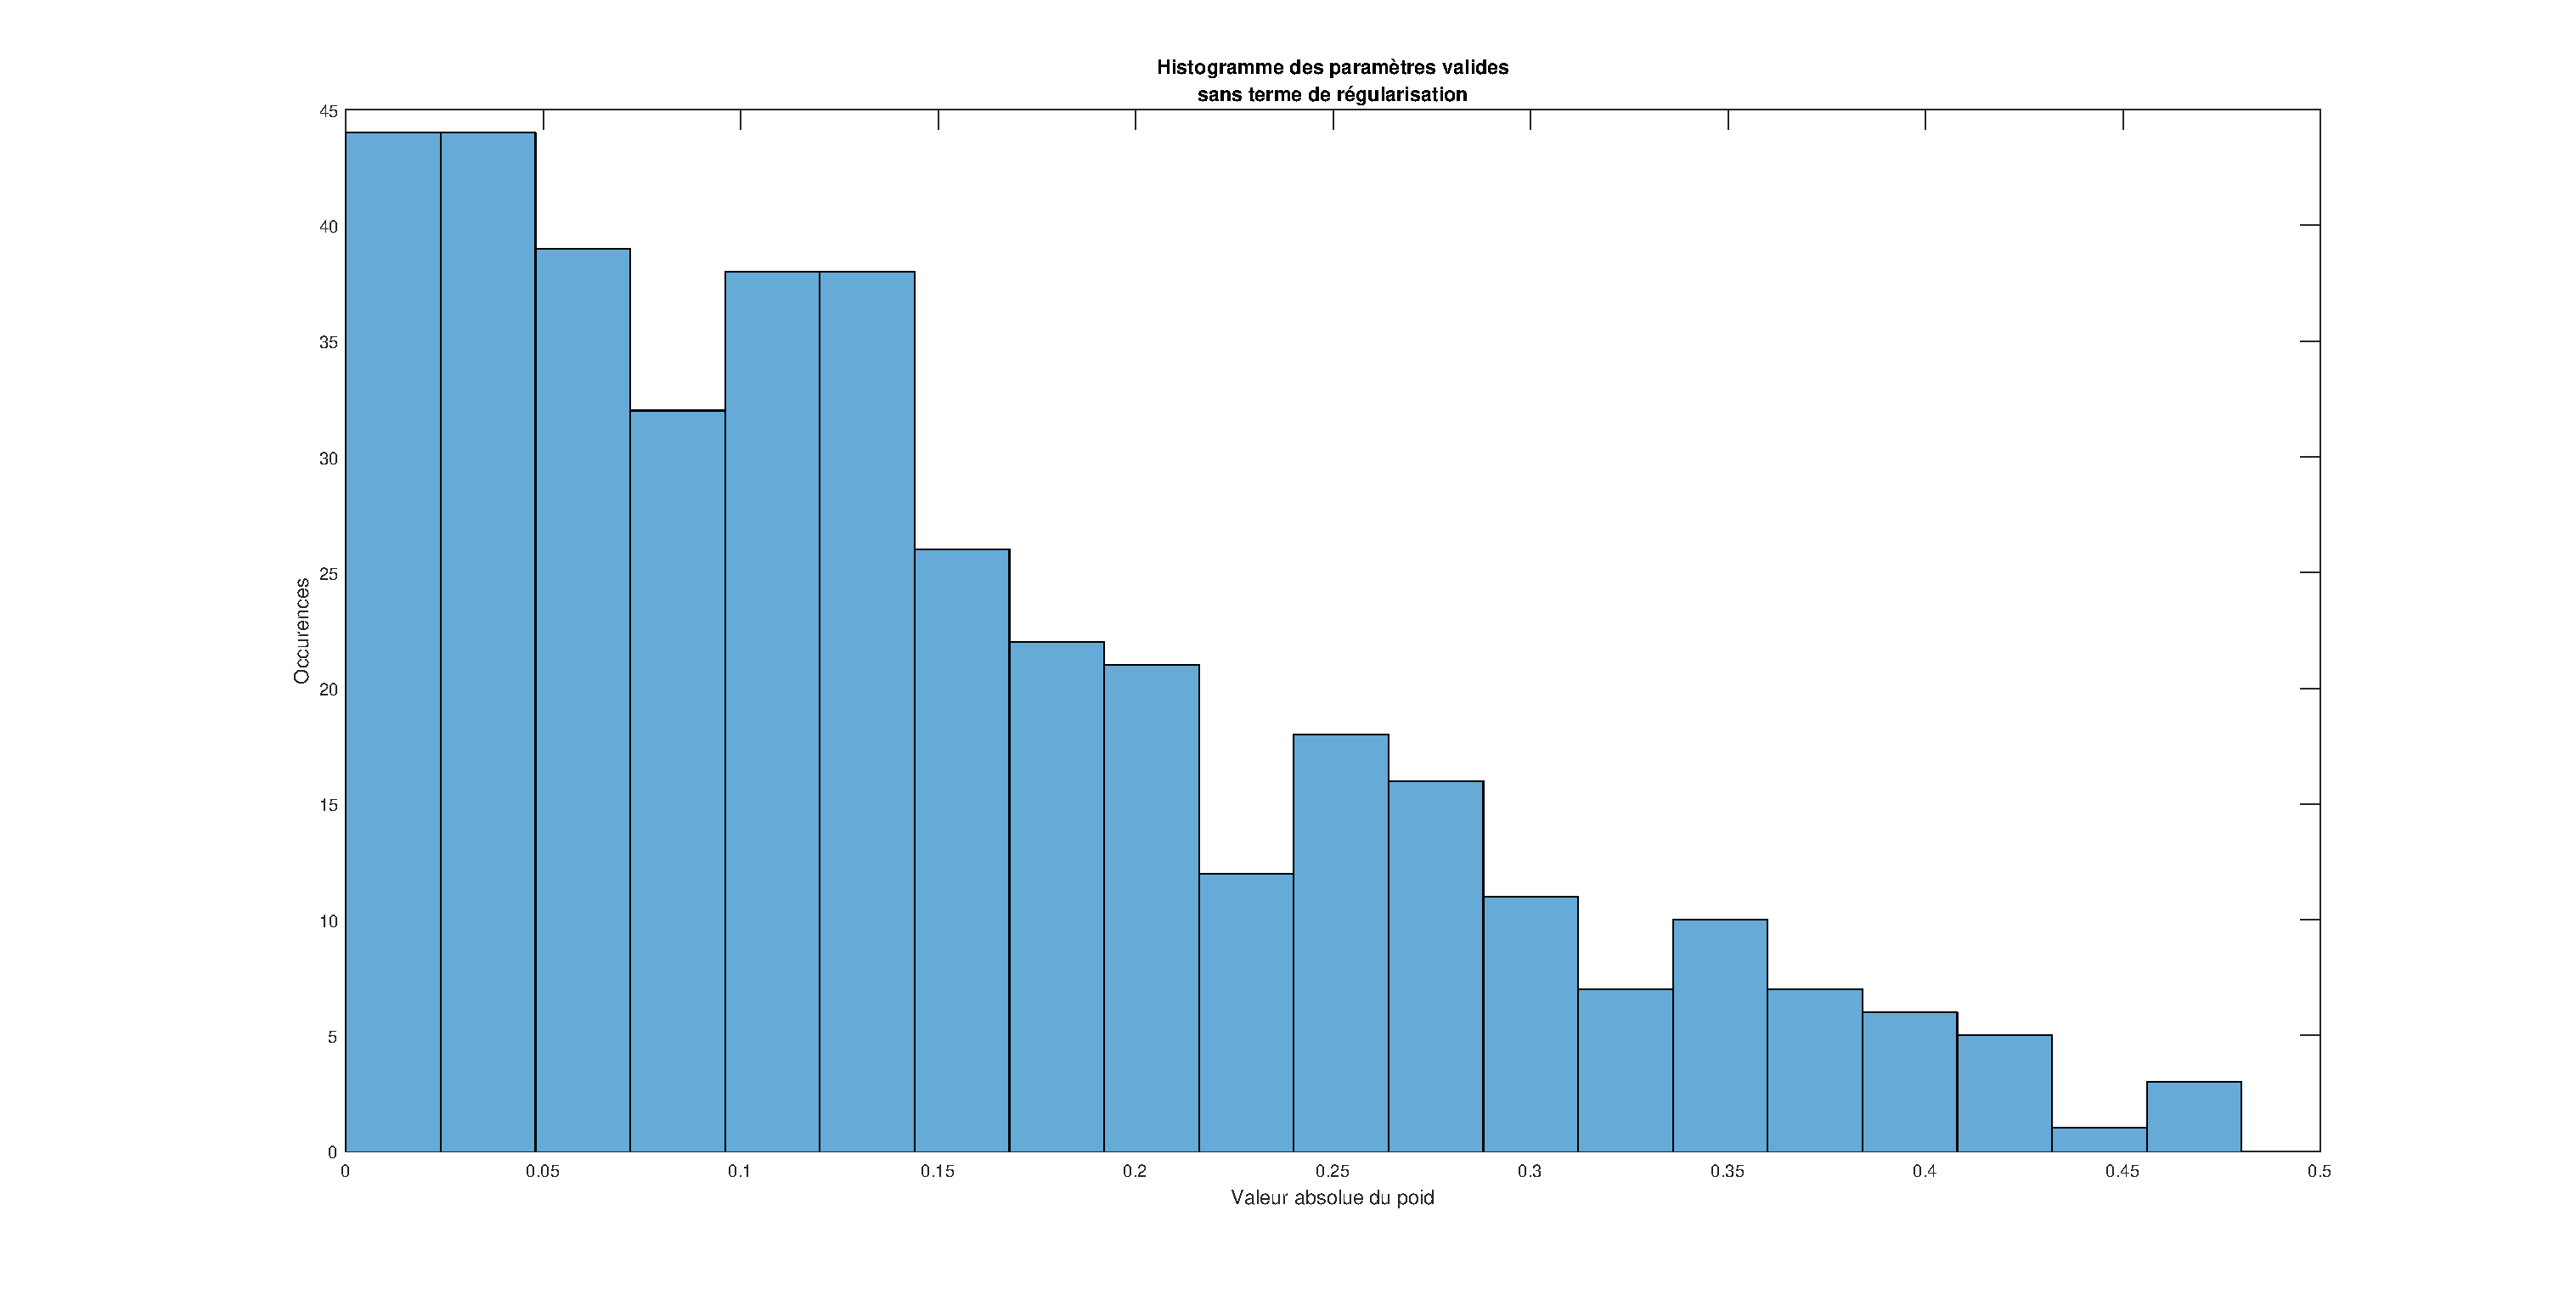
\includegraphics[width=\textwidth,height=\textheight,keepaspectratio]{graphics/histoRandParameterNoRegulation.eps}
\end{figure}

\begin{figure}[H]
\label{randomWeightRegulation}
\caption{Valeur absolue du poids des paramètres aléatoires avec régulation}
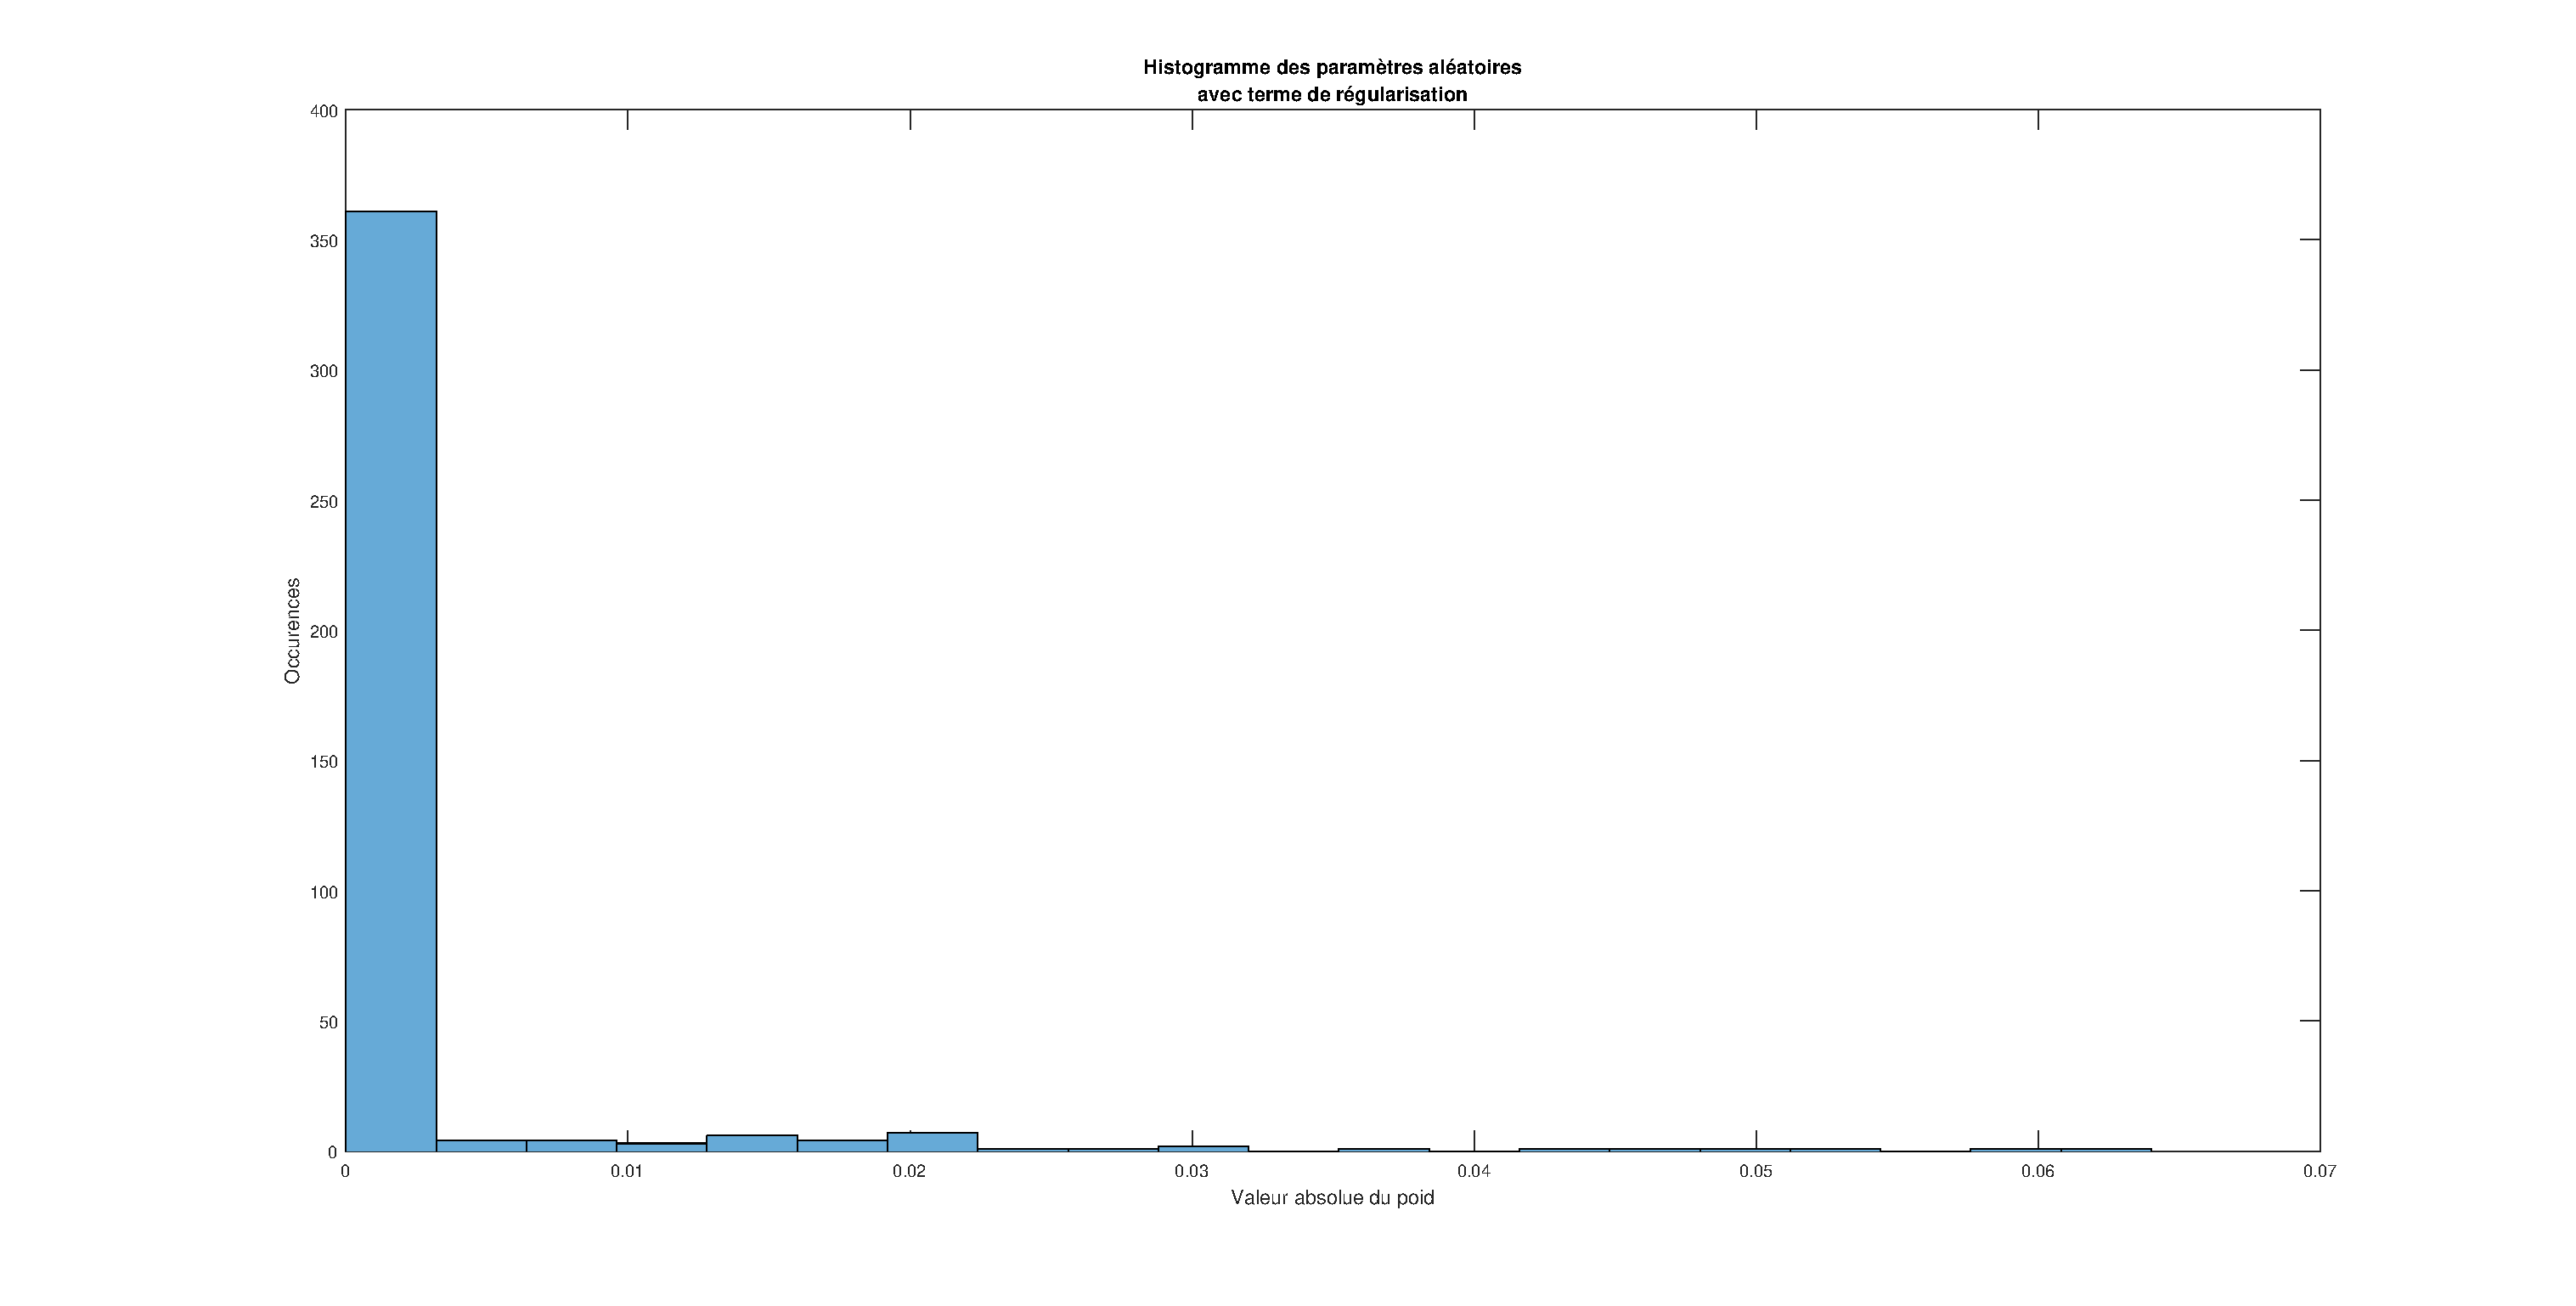
\includegraphics[width=\textwidth,height=\textheight,keepaspectratio]{graphics/histoRandParameterRegulation.eps}
\end{figure}
Comme pour les paramètres valides, les poids des valeurs aléatoires se sont rapproché de 0 grâce au terme de régulation. Aucun des paramètres a un poid supérieur à 0.07 ce qui les rend inutiles pour faire des
prédictions. C'est exactement le résultat attendu car les paramètres aléatoires devraient être distribué de façon uniforme et donc de pas influencer la sortie.
%----------------------------------------------------------------------------------------
\end{document}
\grid
\grid
